\section{Android}

\subsection{Architecture}
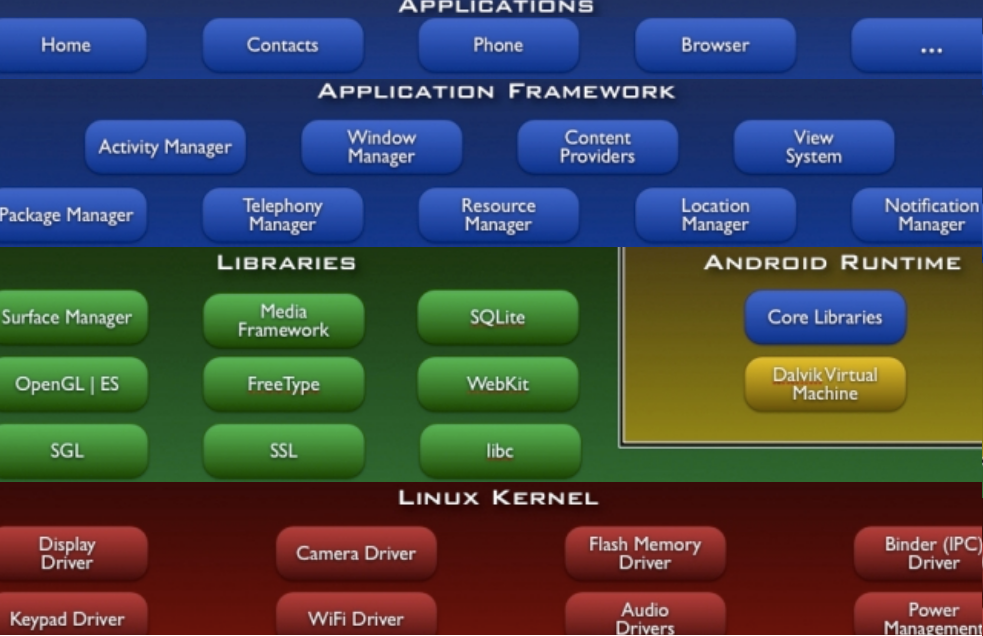
\includegraphics[width=0.15\textwidth]{android/architecture.png}
\textbf{Linux Kernel:} hardware abstraction layer (HAL), device drivers, memory
/ process management, networking

\textbf{Libraries:} C/C++ libraries. Interface through Java. Surface Manager.
2D and 3D Graphics. Media codecs, SQLite, Browser engine

\textbf{Android Runtime:}
Android runtime (ART) and its predecessor Dalvik are the managed runtime used
by apps and some system services.
Executes Dalvik Code (translated from Java bytecode).
Supports Ahead-of-time (AOT) compilation, garbage collections, profiling and
debugging.
Optimized for systems that are constrained in terms of memory and processor
speed.

\textbf{Application Framework:}
API interface, Activity manager (Manages the application life cycle).

\textbf{Applications:}
Built-in and user applications. Can replace built-in applications.

\subsection{Components}
App is built of Components that interacts. Goal: Easy to reuse and replace.
Components of other apps can be used (e.g. Gallery). Needs to be registered in
the AndroidManifest (<activity android:name=".ActivityB" />) (else exception).

\textbf{Activity}
User interface component typically corresponding to one screen. (Moving to next
screen means change of Activity).

\textbf{Service}
Runs in the background without user interface.
Example: music player, network download, etc
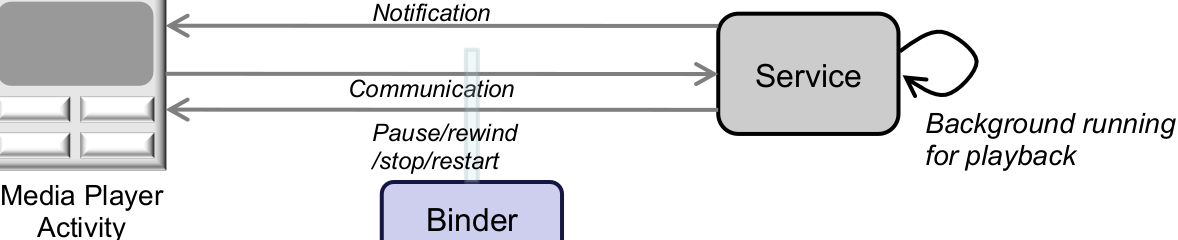
\includegraphics[width=0.15\textwidth]{android/service_example.png}

\textbf{Broadcast Receiver}
Component that receives and reacts to broadcast announcements (<- are Intents too).
Many broadcasts originate in system code (E.g., announcements that the time
zone has changed, that the battery is low. Incoming SMS)
Receiver are implemented by extending BroadcastReceiver.

\textbf{Content Provider}
recommended way to share data between Android applications (E.g. address book,
photo gallery). Represented by URI and MIME type.
Applications do not call content providers directly. They call ContentResolvers
instead as they typically do not reside in the same process.
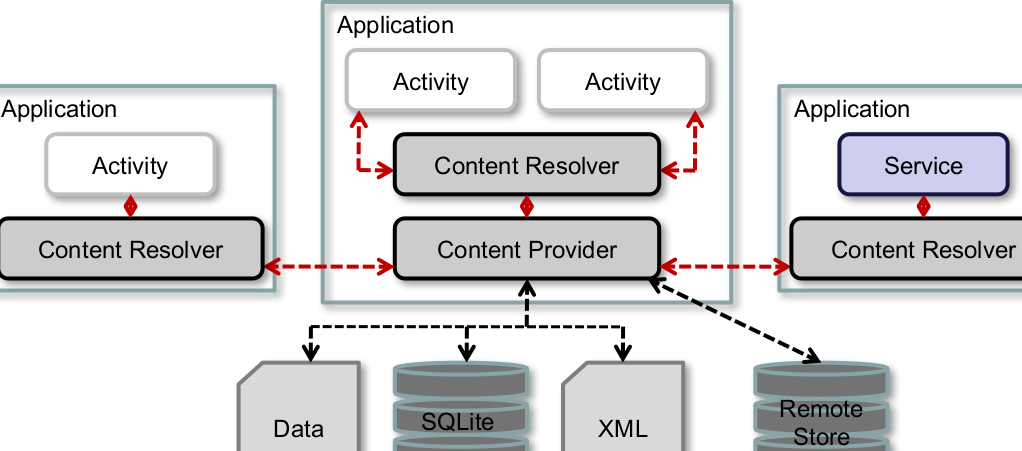
\includegraphics[width=0.15\textwidth]{android/content_provider.png}

\subsection{Processes and Threads}
\textbf{Default:} Applications run in a single Linux process. All components of
an application (activities, services, content providers, etc.) share this
process. These components also share a single thread of execution (“main
thread” or “UI thread”) within this process

\textbf{Processes may get killed} when memory is low. Which one to kill is
decided by an importance hierarchy.
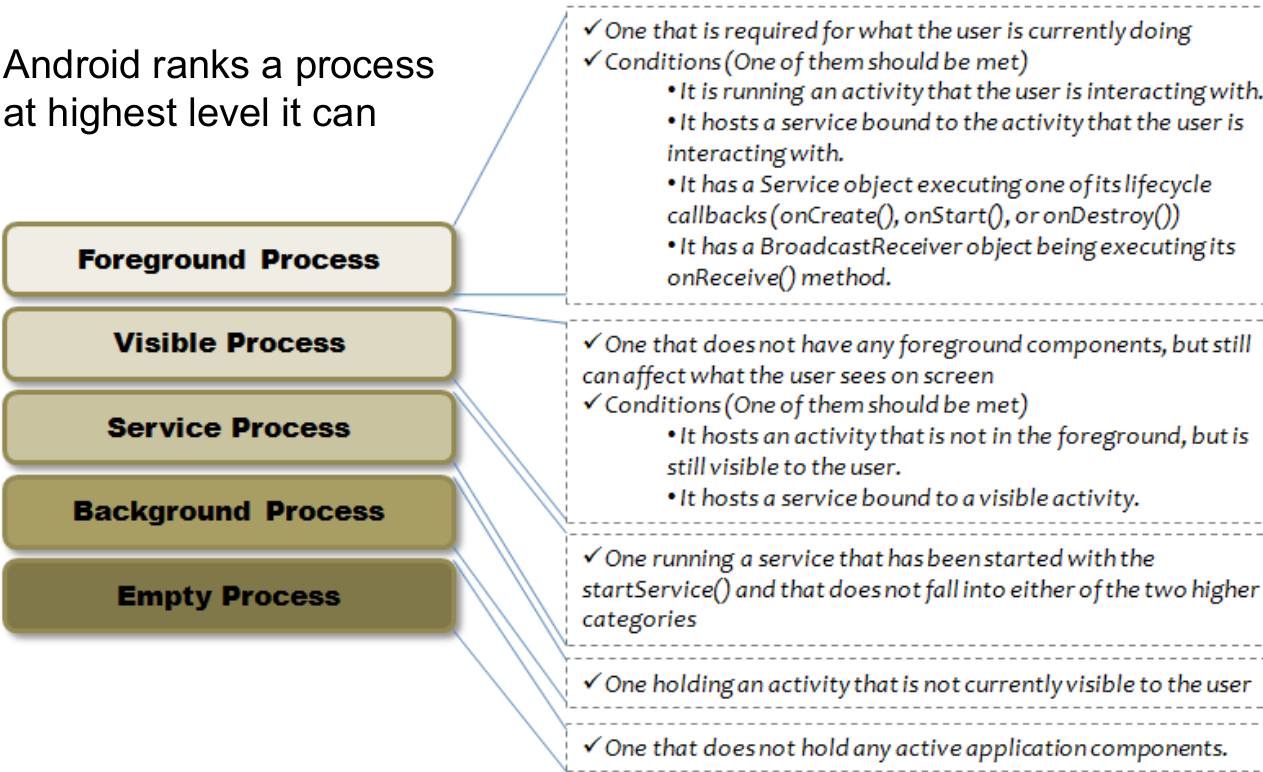
\includegraphics[width=0.15\textwidth]{android/importance_hierarchy.png}

Component ranking may increase if it contains components that serve components
in higher ranked processes. Thus, we recommend to create a service instead of
worker threads.

\textbf{UI Thread} is actually the \textbf{Main Thread}. It is called UI Thread
since all components are instantiated in it. Only this thread is supposed to
interact with the UI toolkit.

\textbf{Worker Thread} for long-lasting-operatins (To avoid infamous
“application not responding”). E.g. computations or downloads. To access
UI-Thread use: Activity.runOnUiThread(Runnable) or View.post(Runnable) or
View.postDelayed(Runnable, long).

\begin{lstlisting}
new Thread(new Runnable() {
public void run() {
 final Bitmap bitmap = load("http://...");
 mImageView.post(new Runnable() {
   public void run() {
    mImageView.setImageBitmap(bitmap);
   }
 });
}
}).start();
\end{lstlisting}

\textbf{Looper} can be used to transform normal thread in continuously running
thread. $prepare()$ transforms thread. $loop()$ starts loop. $quit()$ stops the
loop. The main ui thread is also created with the Looper
(Looper.getMainLooper() returns the looper). Instead of transforming a thread
the \textbf{HandlerThread} class can be used.\\

\textbf{AsyncTask}
Performs operation in background. Results from $doInBackground$ method are sent
to $onPostExecute$ method, which can update the UI Thread. Additionally
supports methods to report progress.

\textbf{Handler}
Can be used to register to a thread and provides a simple channel to send data
to this thread. Create a new instance of the Handler class in the $onCreate()$
method of your activity, the resulting Handler object can be used to transmit
data to the main thread by using: $sendMessage(Message)$ or
$sendEmptyMessage()$. Useful if you want to transmit data multiple times to the
main thread.

\subsection{Storing Data}
Multiple ways to store data are provided:
\subsubsection{Shared Preferences}
Provides a general framework that allows you to save and retrieve persistent
key-value pairs of primitive data types. The data will persist across user
sessions (even if your application is killed). Get Object with
$getPreferences()$ (if you need one file) or $getSharedPreferences()$ if you
need multiple files (distinguished by name).

\textbf{write} values by getting the editor with $edit()$ and call
$putString()$, $putBoolean()$, ... Don't forget to $commit()$ the values.

\textbf{read} with $getBoolean()$, $getString()$, ..

\subsubsection{Internal Storage}
By default, files saved to the internal storage are private to your
application. Other applications cannot access them (nor can the user). When the
user uninstalls your application, these files are removed.

\textbf{write}
\begin{lstlisting}
FileOutputStream fos = openFileOutput(FILENAME, Context.MODE\_PRIVATE);
fos.write(string.getBytes()); fos.close();
\end{lstlisting}

\textbf{read} call $openFileInput()$ with name of file, which returns a
$FileInputStream$. Then $read()$ and $close()$.

\textbf{Static files} Can be saved in res/raw and opened with
openRawResource(), passing the R.raw.<filename> resource ID.

\textbf{Cache files} Employ $getCacheDir()$ before opening. Recommended size <
1 MB. May get deleted when low on space.

\subsubsection{External Storage}
Reading from and writing to external storage (SD card or non-removable storage)
is supported by every Android- compatible device.

check storage availability with $getExternalStorageState$ and access your files
e.g. with $getExternalFilesDir()$.

\textbf{Shared files} getExternalStoragePublicDirectory() passing it the type
of public directory you want such as DIRECTORY\_MUSIC, DIRECTORY\_PICTURES.

\textbf{Cache files} getExternalCacheDir() to get the directory where cache
files can be stored.

\subsubsection{SQLite Databases}
The Android SDK includes a sqlite3 database tool that allows you to browse
table contents. Reads and writes go directly to a single ordinary file (Read /
Write Locks on the entire file).

Use a \textbf{database manager} to create, modify and query a private database.

\begin{lstlisting}
public class EventDBHelper extends SQLiteOpenHelper {
 private static final String DATABASE_NAME = "events.db";
 private static final int DATABASE_VERSION = 3;

 /** Create a helper object for the Events database */
 public EventDBHelper(Context ctx) {
  super(ctx, DATABASE_NAME, null, DATABASE_VERSION);
 }

 //create the database
 @Override
 public void onCreate(SQLiteDatabase db) {
  db.execSQL("CREATE TABLE " + TABLE_EVENTS + " ("
  + _ID + " INTEGER PRIMARY KEY AUTOINCREMENT, "
  + COL_TIME + " INTEGER,"
  + COL_NAME + " TEXT NOT NULL);");
 }

 // called if old version of databse is referenced
 @Override
 public void onUpgrade(SQLiteDatabase db, int oldVersion, int newVersion) {
  db.execSQL("DROP TABLE IF EXISTS " + TABLE_EVENTS);
  onCreate(db);
 }
}
\end{lstlisting}

\textbf{modify data} with either raw queries or \textbf{structured query}
\begin{lstlisting}
// Insert a new record into the Events database
SQLiteDatabase db = eventDBHelper.getWritableDatabase();
// INSERT INTO TABLE_EVENTS (COL_TIME, COL_NAME)
VALUES (System.currentTimeMillis(), string);
ContentValues values = new ContentValues();
values.put(COL_TIME, System.currentTimeMillis());
values.put(COL_NAME, string);
db.insertOrThrow(TABLE_EVENTS, null, values);
\end{lstlisting}

\textbf{querying database (windowing)} prevents the system from having to load
all result data at a time and thus saves memory. Generally, cursors need to be
closed. A cursor can be registered at the Activity that performs the query. As
a consequence the Android system handles closing and re-querying when needed as
after lifecycle events such as onPause.

\subsubsection{Network Connection}
To send and receive data you may employ the class HttpURLConnection.
Alternatively you may employ libraries such as Gson and OkHttp.

\begin{lstlisting}
URL url = new URL("http://www.android.com/");
HttpURLConnection urlConnection = (HttpURLConnection)
url.openConnection();
try {
  InputStream in = new BufferedInputStream(urlConnection.getInputStream());
  readStream(in);
  finally {
    urlConnection.disconnect();
  }
}
\end{lstlisting}

\subsection{Transferring Program Control / Intents}
\textbf{Intents:} (Passive object, Set of Strings). Used for transfering
control or notify components (VIEW, CALL, PLAY, ...). Systems matches Intent
with most suitable. It can be used to start an activity, start or communicate
with background service, send broadcast

\begin{lstlisting}
public void onClickSendBtn(final View btn){
  Intent intent = new Intent(this, Receiver.class);
  intent.putExtra("msg", "Hello World");
  startActivity(intent);
}
\end{lstlisting}

\textbf{Explicit Intent:} fully qualified class name of target. Mostly used for
internal messages of an application (starting an activity).

\textbf{Implicit Intent:} passive data structure holding an description of an
action to be performed. \textit{Action}: e.g. ACTION\_VIEW, ACTION\_EDIT.
\textit{Category:} category of component that should handle the intent (e.g.
browsable). \textit{Data:} URI and data type (MIME type). \textit{Extras}
Key-value pairs for additional information.

To \textbf{handle implicit intents} define intent filters in AndroidManifest.
Components without a filter can only receive explicit intents.

System \textbf{resolves implicit intent} by matching the most suitable
component (action, category, data). If multiple components match the filter,
the user can chose. If no component match, an exception is raised.

\textbf{resolution rules:}

\textit{Action}: if intent and filter has no action => fails. If filter has
action but intent not => match.

\textit{Category}: Every category of intent must match (but filter can contain
more)! DEFAULT is necessary to receive implicit intents. LAUNCHER category is
necessary if callable from launcher.

\textit{Data}: if 1) intent contains type and URI (or type can inferred from
URI) => filter matches if type and URI are the same.
2) Intent contains either type nor URI => filter matches if no type and URI are
defined
3) Intent contains URI but no type (and type can not be inferred) => filter
matches if URI matches and no type is defined.
4) Intent contains type but no URI => filter matches if type matches and no URI defined


\textbf{E.g. of Intent Filter in AndroidManifest}
\begin{lstlisting}
<activity android:name="SomeActivity">
  <intent-filter>
      <action android:name="android.intent.action.EDIT" />
      <category android:name="android.intent.category.DEFAULT" />
      <data android:scheme="http" android:type="video/*" />
  </intent-filter>
</activity>
\end{lstlisting}

Android uses a requestId to \textbf{return results from a sub-activity}:
\begin{lstlisting}
startActivityForResult(new Intent(this, A.class), i1);
startActivityForResult(new Intent(this, B.class), i2);

// in sub-activity A or B
setResult(resultCode, intent); finish();

// back in main activity
@Override
protected void onActivityResult(int requestCode, int resultCode, Intent
data) {
  switch (requestCode) {
    case i1: // result from call with i1
    if (resultCode == RESULT_OK) { /* ... */ }
    break;
    case i2: // result from call with i2
    if (resultCode == RESULT_OK) { /* ... */ }
    break;
  }
}
\end{lstlisting}



\subsection{Activity Lifecycle}
State of an activity is managed by the system.

System may:
1) move another activity into the foreground.
2) ask the activity to finish.
3) even simply kill its process.

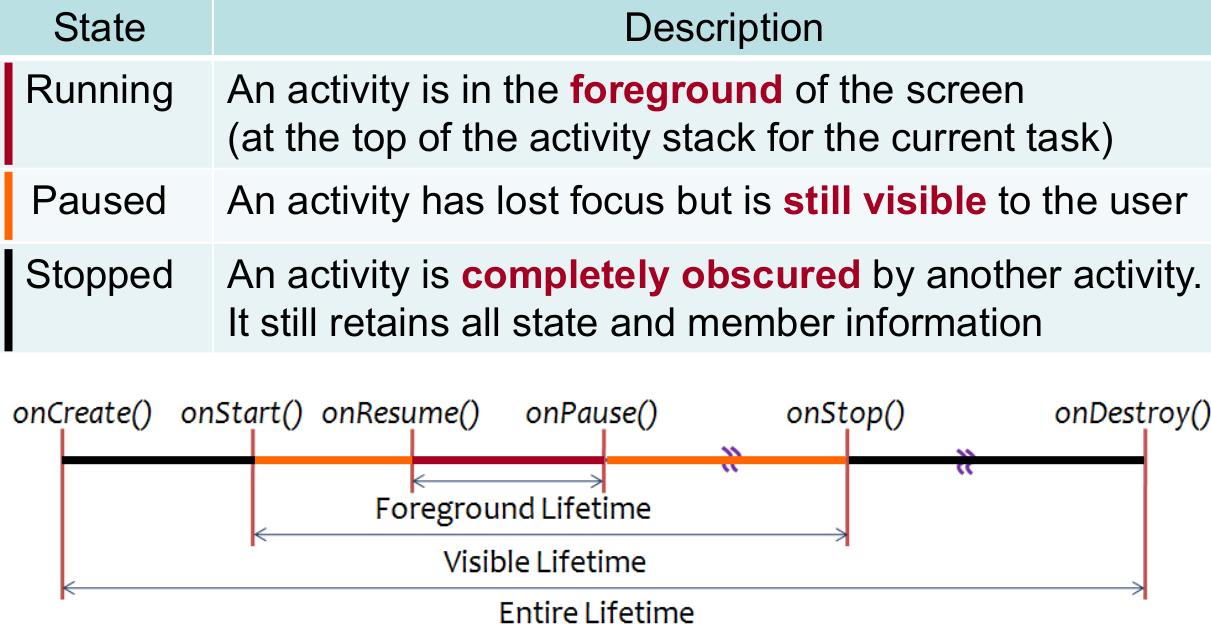
\includegraphics[width=0.15\textwidth]{android/activity_states.png}
System notifies an activity of a state transition by calling methods:
\textbf{onCreate:} first create or when activity was killed.
\textbf{onStart:} just before activity becomes visible.
\textbf{onRestart:} after activity has been stopped, to being started again.
\textbf{onResume:} before activity starts interacting with user (input goes to activity).
\textbf{onPause:} when about to resuming other activity (commit unsaved changes
here! stop animiations and CPU consumings)
\textbf{onStop:} when no longer visible to user (e.g. when destroyed or other activity resumed)
\textbf{onDestroy:} before destroy, but there is no guarantee.


\subsection{AndroidManifest}
Properties of Application: Name / ID (package), Version of App, Technical User
(sharedUserId), Required SDK, Required Privileges, Components
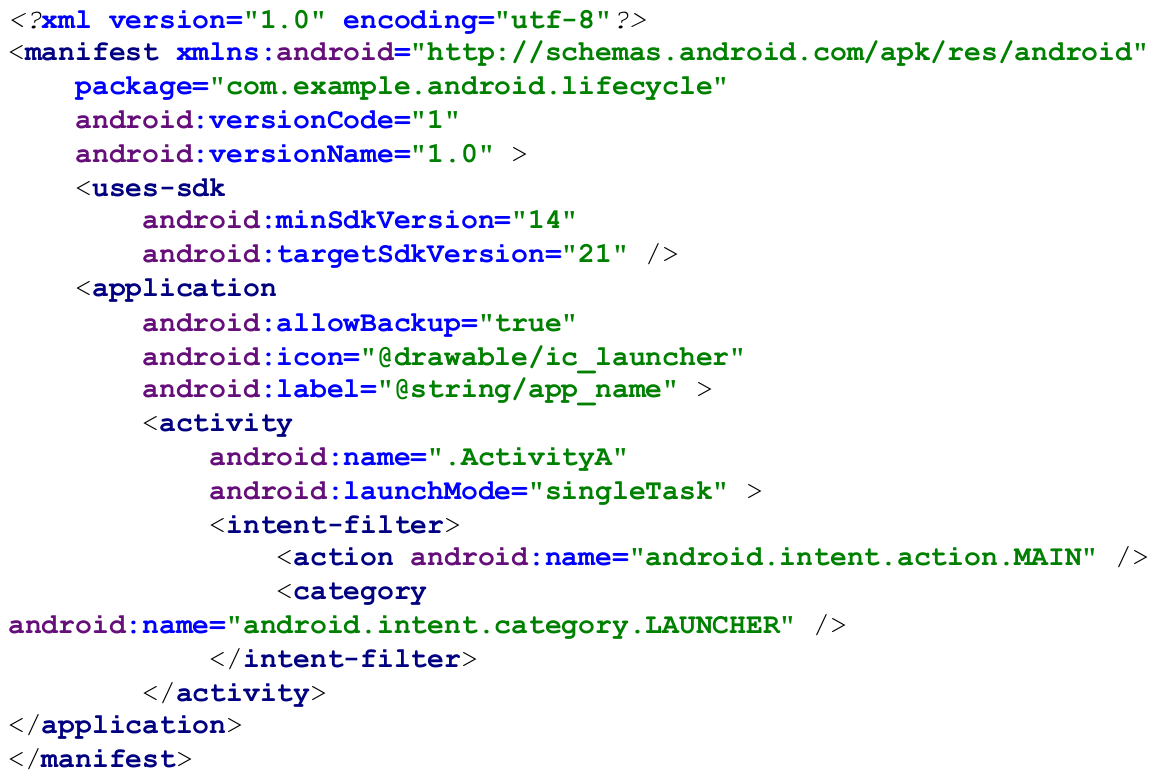
\includegraphics[width=0.15\textwidth]{android/manifest.png}
To be available from the launcher it must include an intent filter listening
for the MAIN action and the LAUNCHER category

\subsection{Configuration}
Advantages: Strings for localization, Images for different resolutions, Layouts for
different devices, ...

Seperated from code with resource files. Stored in \textbf{res} directory and
grouped by type: \textit{drawable}, \textit{layout}, \textit{values}. For
example \textit{res/values-de/strings.xml}
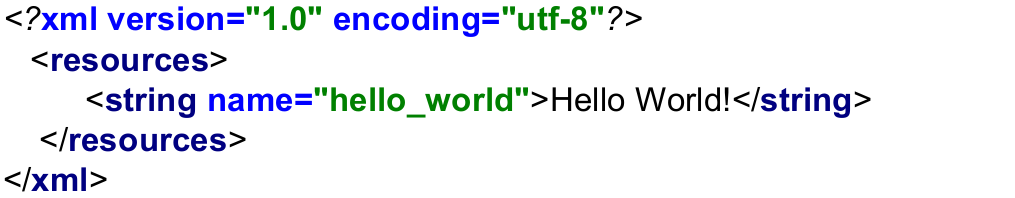
\includegraphics[width=0.15\textwidth]{android/example_resource.png}

Accessing resources in Java code with \textbf{wrapper class called R}, that
contains resource ids as static integers.

\begin{lstlisting}
// Load a custom layout for the current screen
setContentView(R.layout.main_screen);
// Set the text on a TextView object.
TextView view = (TextView)findViewByID(R.id.msg);
msgTextView.setText(R.string.hello_message);
// Set the title from a resource
this.getWindow().setTitle(Resources.getText(R.string.main_ title));
// Load a background for the current screen from a resource
this.getWindow().setBackgroundDrawableResource(R.drawable.my_background_image);
\end{lstlisting}

\subsection{Layout}
Defines the elements and their positioning on the user interface. Elements can
be declared in Java or XML. Advantages XML: seperation of presentation code.

Layout composed of \textbf{View} and \textbf{ViewGroups} (LinearLayout,
RelativeLayout, TableLayout, Gridlayout). ViewGroup contains other Views. Views
for interaction with User are called \textbf{Widgets} (Buttons, Check Boxes,
...). Good practice is to declare Layouts and UI elements in XML and to
instantiate them by creating Views and ViewGroups at run time.

Each view must define height and width with \textit{wrap\_content} or
\textit{fill\_parent}.
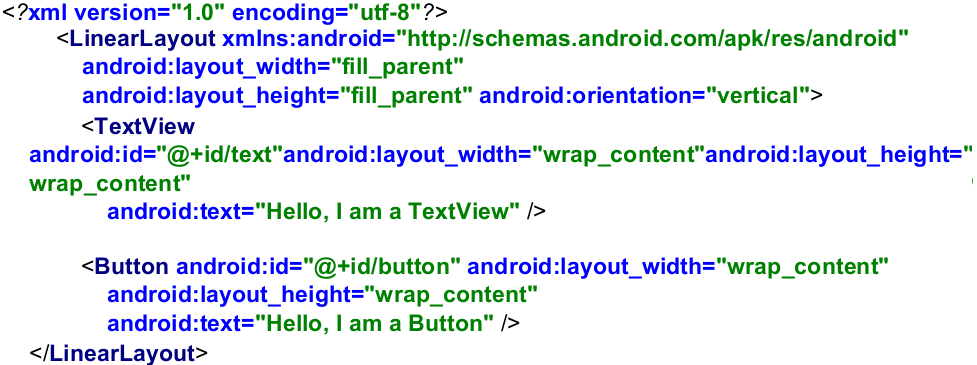
\includegraphics[width=0.15\textwidth]{android/view_example.png}

Handling UI Events like in Java Swing:
\begin{lstlisting}
// Capture our button from layout
Button button = (Button)findViewById(R.id.corky);
// Register the onClick listener with the impl. abovE
button.setOnClickListener(mCorkyListener);
\end{lstlisting}

\subsection{Development}
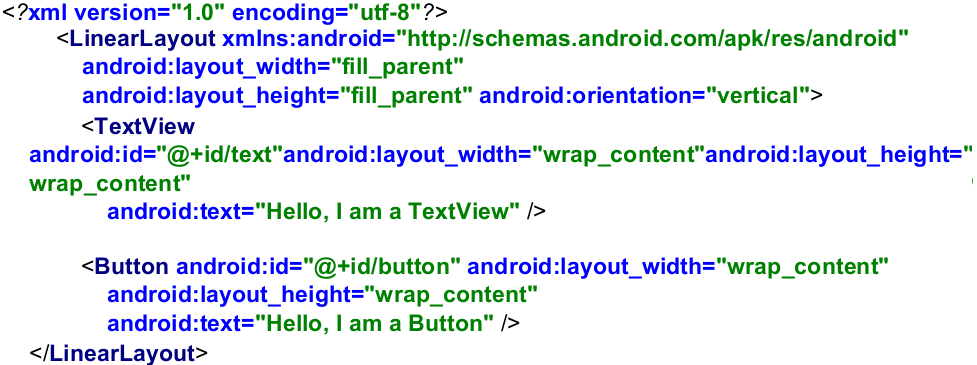
\includegraphics[width=0.15\textwidth]{android/view_example.png}
\textbf{Minimum Required SDK:} lowest version app supports.
\textbf{Target SDK:} Highest version app is tested for.
\textbf{Compile With:} Version against app is compiled.
\textbf{Theme:} Specific Android UI Theme.

\subsection{List}
ListActivity displays items by binding to a data source (\textbf{adapter}:
array, cursor). It consists of screen and row layout.
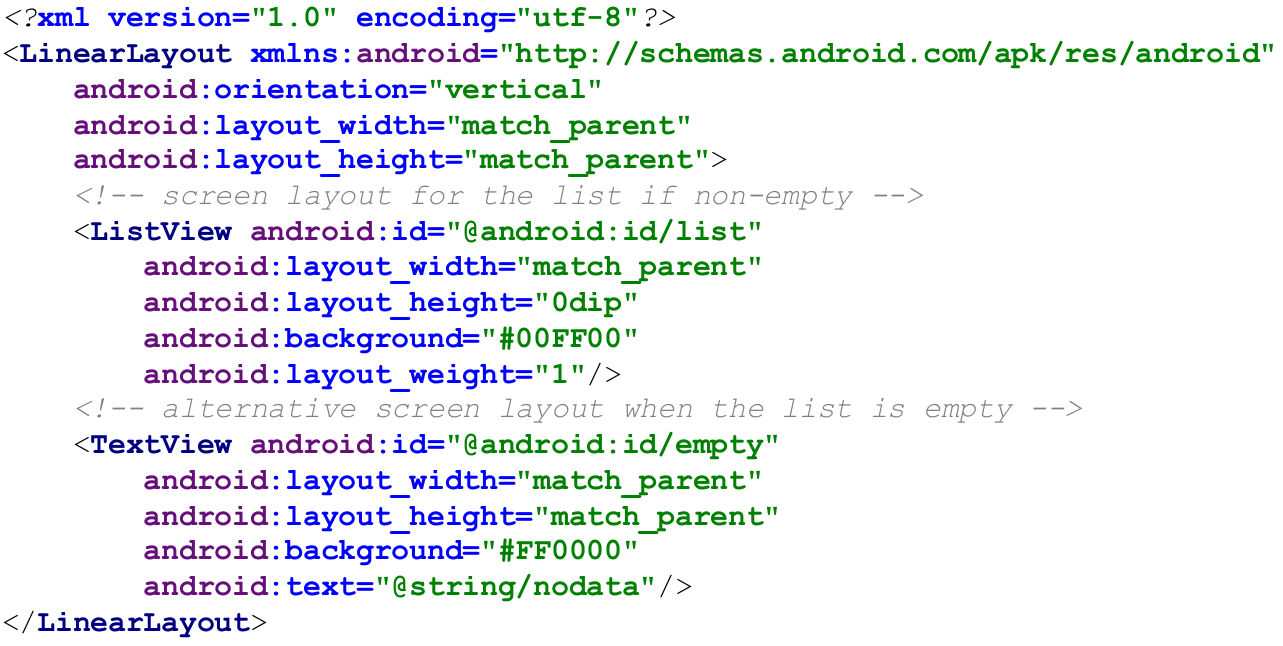
\includegraphics[width=0.15\textwidth]{android/list_layout_example.png}

Row Layout is defined when setting adapter. Define a own row layout or use
predefined built-in layouts (e.g. R.layout.simple\_list\_item\_1):
\begin{lstlisting}
setListAdapter(new ArrayAdapter<String>(this,
android.R.layout.simple_list_item_1, mValues););
\end{lstlisting}

onListItemClick:
\begin{lstlisting}
protected void onListItemClick(ListView l, View v, int position, long id)
\end{lstlisting}

To improve the \textbf{Performance} the \textbf{ViewHolder} pattern can be
used. It avoids frequent call of $findViewById$ during scrolling.
\begin{lstlisting}
static class ViewHolder { TextView text; }
@Override
public View getView(int position, View convertView, ViewGroup parent) {
  if(convertView==null){
    LayoutInflater inflater = ((Activity) mContext).getLayoutInflater();
      convertView = inflater.inflate(layoutResourceId, parent, false);
      viewHolder = new ViewHolderItem();
      viewHolder.text = (TextView) convertView.findViewById(R.id.textViewItem);
      convertView.setTag(viewHolder);
    } else { viewHolder = (ViewHolderItem) convertView.getTag(); }
    // modify value of viewHolder
}
\end{lstlisting}


\subsection{Recycler View}
more sophisticated alternative to display lists and grids (Fast scrolling
through large lists, Items are added or removed at run-time, Item add or
removal is to be animated)

Optimizations and enhancements come from:
1) a ViewHolder inner class in the adapter holding references to the views of
an individual item.
2) use of notification methods for item add or removal
3) possibilites to define animations by overwriting classes such as
RecyclerView.ItemAnimator

\subsection{Fragments}
Fragments are small chunks of the UI. They have their own layout and can be
inserted to an activity (by adding <fragment> element to the activity
declaration in XML, or from Java code by adding it to an existing ViewGroup).

\textbf{Advantages:} Can be reused in multiple activities. They have their own
\textit{backstack} and \textit{lifecycle} (usually implement at least:
onCreate, onCreateView and onPause).

\textbf{Example}
To show more details in landscape use create a xml layout for both orientations
(with same name). Landscape contains $android:orientation="horizontal"$ and a
FrameLayout for details:
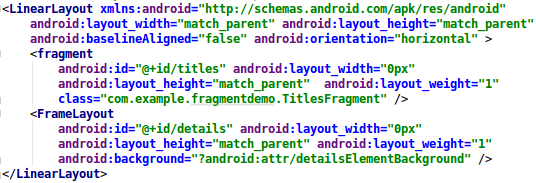
\includegraphics[width=0.15\textwidth]{android/fragment_details.png}

Check in ListFragment if details element is visible and use
\textbf{FragmentManager} to set it:
\begin{lstlisting}
public class TitlesFragment extends ListFragment {
  // check if details fragment visible
  View detailsFrame = getActivity().findViewById(R.id.details);
  landscape = detailsFrame != null && detailsFrame.getVisibility() == View.VISIBLE;
  // create details fragment if landscape is true
  details = DetailsFragment.newInstance(index);
  FragmentTransaction ft = getFragmentManager().beginTransaction();
  ft.replace(R.id.details, details);
  ft.setTransition(FragmentTransaction.TRANSIT_FRAGMENT_FADE);
  ft.commit();
\end{lstlisting}

\textbf{Useful subclasses of Fragments:}
\textit{DialogFragment} (Floating Dialog. Good alternativ to default Dialog,
since it works with back-stack).  \textit{ListFragment}.
\textit{PreferenceFragment} (Displays a hierarchy of Preference objects as a
list, Follows the visual style of system preferences).

\textbf{Communication:}
To be modular and decoupled any communication between fragments needs to go
through the hosting activity. To decouple communication fragment defines
interface which the activity implements:

\begin{lstlisting}
public class MyListFragment extends ListFragment {
  private OnItemSelectedListener listener;
  public interface OnItemSelectedListener {
    public void onRssItemSelected(String link);
  }
  public void onAttach(Activity activity) {
    super.onAttach(activity);
    listener = (OnItemSelectedListener) activity;
  }
  public void onListItemClick(ListView l, View v, int position, long id) {
    String title = l.getItemAtPosition(position).toString();
    RssItem rssItem = list.get(position);
    listener.onRssItemSelected(rssItem.getTitle());
    super.onListItemClick(l, v, position, id);
  }
\end{lstlisting}

\subsection{Application Menus}
Three types: Options menu, Context menu, Popup menu

\subsection{Android Action Bar}
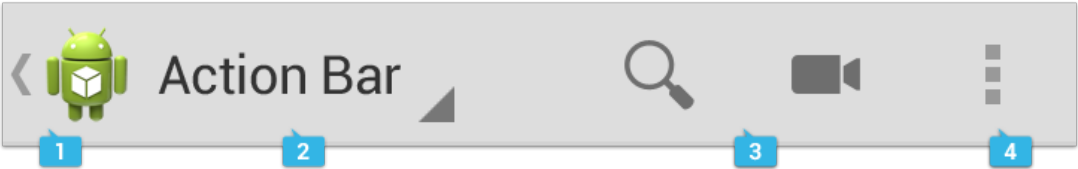
\includegraphics[width=0.15\textwidth]{android/actionbar.png}
1) app icon
2) view control
3) action button
4) overflow button

\textbf{Guidelines for Action Buttons}
Order by importance. Standard icons. Consider frequent, important and typical
actions. Buttons should not take more than 50\% of width. Not too many icons.

\textbf{Fragments} may contribute actions buttons with $hasOptionsMenu$ in
$onCreate$. Android calls $onCreateOptionsMenu$ in the fragment.

\newpage
\subsection{TODO SOME QUESTIONS OF BSKON EXAMS BECAUSE SAME TEACHER AND SAME CONTENT}
